\documentclass[11pt]{article}

\usepackage[margin=1in]{geometry}
\usepackage{amsmath,amssymb}
\usepackage{graphicx}
\usepackage{booktabs}
\usepackage{array}
\usepackage{xcolor}
\usepackage{algorithm}
\usepackage{algpseudocode}
\usepackage{natbib}
\usepackage[colorlinks=true,linkcolor=blue,citecolor=blue,urlcolor=blue]{hyperref}

\title{\textbf{Auto Dataset Builder: An Automated Annotation Framework\\
with Vision-Language Verification and Neural Dataset Quality Scoring}}

\author{
Yu-Wei Chen \\
Bachelor Program of Intelligent Robotics \\
National Yunlin University of Science and Technology \\
\texttt{chenchen931209@gmail.com}
}

\date{}

\begin{document}

\maketitle

\begin{abstract}
The construction of high-quality training datasets remains a primary bottleneck
in computer vision model development, with annotation reportedly consuming
60--80\% of project time. We present \textbf{Auto Dataset Builder (ADB)}, an
automated framework that converts unlabeled images into YOLO-compatible
annotated datasets through a three-stage pipeline: (1) YOLOv11 proposal
generation, (2) SAM2 mask-guided bounding-box refinement, and (3) zero-shot
semantic verification, for which the framework supports either a Vision-LLM
backend (Qwen-VL-Chat / LLaVA) or a CPU-friendly CLIP ViT-B/32 zero-shot
classifier. We additionally introduce the \textbf{Neural Dataset Quality
Score (Neural DQS)}, a lightweight regressor that estimates the expected
mAP@0.5 a YOLOv11 model will achieve after training on a given dataset, computed from
six interpretable dataset-level features without requiring any model
training. On 96 controlled degradation variants of COCO128, Neural DQS
achieves a 5-fold cross-validated Pearson correlation of $r=0.929$
($R^2=0.854$, $p<0.001$) with actual mAP@0.5; ablation and SHAP analyses
identify CLIP-space semantic diversity as the dominant predictor, with its
removal dropping $r$ to $0.679$. On a 597-image COCO2017 motorcycle subset,
ADB's fully automated annotations reach 94.2\% of the mAP@0.5 obtained from
human (Manual) annotations (0.441 vs.\ 0.468) with zero manual labeling
effort. A single active-learning iteration (ADB+AL), which re-annotates the
100 most uncertain images from a held-out unlabeled pool, closes this gap
entirely and matches the strongest baseline at mAP@0.5$=0.476$. Code is
available at
\url{https://github.com/ericchen931209/auto-dataset-builder}.
\end{abstract}

\section{Introduction}

\subsection{Motivation}

The performance of modern object detection systems is determined as much by
the quality of their training data as by model architecture. Yet dataset
construction --- collection, annotation, cleaning, and quality control ---
remains the most labor-intensive part of the machine learning pipeline.
Weak-supervision frameworks such as Snorkel were motivated precisely by the
observation that hand-labeling training data is the dominant cost of
building a new model~\citep{ratner2017snorkel}. Even after labels are
produced, they are frequently noisy: large-scale audits of widely used
benchmark datasets have found that a non-trivial fraction of labels are
incorrect, motivating tools for systematic label-error detection such as
confident learning~\citep{northcutt2021confident}. At the same time,
empirical scaling studies show that detection and classification performance
continues to improve approximately log-linearly with the amount of training
data well beyond the scale of standard academic benchmarks
~\citep{sun2017revisiting}. Together, these findings suggest that
\emph{automating} dataset construction --- while preserving label quality ---
is one of the highest-leverage problems in applied computer vision.

\subsection{Problem Statement}

Existing approaches to dataset construction each address only part of this
problem:

\begin{enumerate}
\item \textbf{Semi-automatic annotation tools} (e.g., CVAT, LabelImg,
  Supervisely) provide efficient interfaces for human annotators but still
  require substantial manual effort per image.
\item \textbf{Synthetic data generation} (GANs, diffusion models) can produce
  unlimited labeled images, but suffers from a persistent domain gap between
  synthetic and real-world distributions.
\item \textbf{Public datasets} (e.g., COCO, ImageNet, YFCC100M) provide
  large-scale, pre-labeled data, but rarely match the class vocabulary,
  geography, or visual conditions of a specific deployment scenario.
\item \textbf{Data flywheel systems} deployed by industrial players (e.g.,
  Tesla, Scale AI) close this gap by continuously re-annotating
  model failures, but require large-scale deployment infrastructure that is
  inaccessible to most research groups and small teams.
\end{enumerate}

What is missing is an open, reproducible, end-to-end pipeline that takes a
collection of unlabeled images for a target object class and produces an
annotated, training-ready dataset --- together with a principled way to
\emph{measure} whether that dataset is good enough to train a useful model,
without first paying the cost of training.

\subsection{Contributions}

We make the following contributions:

\begin{enumerate}
\item \textbf{ADB Framework}: an open-source, end-to-end system that takes a
  natural-language dataset request and a pool of unlabeled images and
  produces a cleaned, quality-scored, YOLO-compatible annotated dataset,
  combining data collection, deduplication, cleaning, automated annotation,
  quality scoring, and active learning into a single pipeline.
\item \textbf{Three-Stage Annotation Pipeline}: a pipeline that combines
  YOLOv11 proposal generation, SAM2 bounding-box refinement, and zero-shot
  semantic verification (Vision-LLM or CLIP), providing both geometric and
  semantic correctness guarantees without any human-in-the-loop annotation.
\item \textbf{Neural DQS}: a learned, interpretable Dataset Quality Score
  that predicts post-training mAP from six dataset-level features, validated
  with a cross-validated Pearson correlation of $r=0.929$ against ground-truth
  mAP, and analyzed with SHAP for feature-level interpretability.
\item \textbf{Active Learning Integration}: an uncertainty-driven active
  learning loop that uses the same three-stage pipeline to automatically
  re-annotate the most informative unlabeled images, closing the performance
  gap to fully manual annotation.
\end{enumerate}

\subsection{Paper Organization}

Section~\ref{sec:related} reviews related work on automated data collection,
semi-automatic annotation, dataset quality assessment, and active learning.
Section~\ref{sec:adb} presents the ADB framework architecture and the
three-stage annotation pipeline. Section~\ref{sec:dqs} formalizes the Neural
DQS model. Section~\ref{sec:al} describes the active learning component.
Section~\ref{sec:experiments} presents experimental results on both Neural
DQS correlation and end-to-end ADB system comparison. Section~\ref{sec:conclusion}
concludes with limitations and future work.

\section{Related Work}
\label{sec:related}

\subsection{Automated Data Collection}

Large-scale image and video collection pipelines such as
YFCC100M~\citep{thomee2016yfcc100m} and Sports-1M~\citep{karpathy2014large}
demonstrated that web-scale media can be harvested and filtered into useful
training corpora, but typically rely on weak metadata (tags, titles) rather
than verified object-level annotations. More recent academic pipelines build
on tools such as \texttt{yt-dlp} to extract domain-specific video frames,
followed by deduplication and manual or semi-automatic labeling. ADB follows
this collection-then-annotate paradigm but automates the annotation step
end-to-end.

\subsection{Semi-Automatic Annotation}

Tools such as CVAT, LabelImg, and Supervisely keep a human annotator in the
loop, using model-assisted suggestions to reduce per-box annotation time but
not eliminate it. The introduction of foundation models for segmentation,
most notably the Segment Anything Model
(SAM)~\citep{kirillov2023segment} and its video-capable successor
SAM2~\citep{ravi2024sam2}, enables prompt-based, zero-shot mask generation
from a single bounding-box or point prompt. ADB uses SAM2 as a
\emph{refinement} stage: rather than generating proposals from scratch, it
tightens detector-generated bounding boxes into pixel-accurate masks and
re-derives bounding boxes from those masks.

\subsection{Dataset Quality Assessment}

Cleanlab's confident learning framework~\citep{northcutt2021confident}
identifies likely label errors in an existing dataset via the disagreement
between a model's predicted and given labels. Dataset
Cartography~\citep{swayamdipta2020dataset} characterizes individual training
examples by their training dynamics (confidence and variability across
epochs), distinguishing ``easy'', ``hard'', and ``ambiguous'' examples.
DataPerf~\citep{mazumder2022dataperf} provides standardized benchmarks for
comparing data-centric algorithms across tasks. These approaches are largely
\emph{post-hoc}: they analyze a dataset (or per-example training dynamics)
after annotation and, in the case of Dataset Cartography, after at least
partial training. In contrast, Neural DQS is computed directly from
dataset-level statistics --- without training a model --- and is explicitly
trained to predict the \emph{downstream mAP} that a detector will achieve,
giving a single scalar, actionable signal before any training occurs.

\subsection{Active Learning}

Classical active learning selects the most informative unlabeled examples
for annotation using criteria such as uncertainty
sampling~\citep{lewis1994sequential}, core-set
selection~\citep{sener2018active}, or a combination of uncertainty and
diversity as in BADGE~\citep{ash2020deep}. ADB's active learning loop
(Section~\ref{sec:al}) uses a simple max-confidence uncertainty criterion,
but differs from prior work in its \emph{termination condition}: rather than
iterating for a fixed budget or until a labeling budget is exhausted, the
loop is designed to terminate when the Neural DQS of the augmented dataset
exceeds a target quality threshold $\theta_q$, tying the active learning
loop directly to predicted downstream performance rather than model
uncertainty alone.

\section{Method --- ADB Framework}
\label{sec:adb}

\subsection{System Overview}

ADB is organized as a pipeline of nine stages, summarized in
Table~\ref{tab:modules}. The system accepts a dataset request --- either a
natural-language description (e.g., ``Build a motorcycle detection
dataset'') or an explicit specification of target classes --- and produces a
versioned, exportable, quality-scored dataset.

\begin{table}[h]
\centering
\caption{ADB pipeline stages.}
\label{tab:modules}
\begin{tabular}{@{}cll@{}}
\toprule
Stage & Module & Function \\
\midrule
1 & Request Parsing & Parse a dataset request into target classes, region, and sample-size constraints \\
2 & Planning & Expand search keywords and define the annotation schema (YOLO/COCO) \\
3 & Collection & Crawl images/video (\texttt{yt-dlp}, image search) and remove near-duplicates \\
4 & Frame Extraction & Extract frames from video at fixed or adaptive (SSIM-based) rates \\
5 & Annotation & Three-stage pipeline: YOLOv11 $\to$ SAM2 $\to$ zero-shot verification \\
6 & Cleaning & Remove blurry, dark, or overexposed images \\
7 & Quality Scoring & Compute Neural DQS$(D)$ from six dataset-level features \\
8 & Active Learning & Re-annotate the most uncertain pool images and merge into $D$ \\
9 & Export & Export to YOLO or COCO format with versioned manifests \\
\bottomrule
\end{tabular}
\end{table}

This paper focuses its empirical evaluation on the components most directly
responsible for dataset quality and downstream model performance: the
three-stage annotation pipeline (Stage 5, Section~\ref{sec:pipeline}), Neural
DQS (Stage 7, Section~\ref{sec:dqs}), and the active learning loop (Stage 8,
Section~\ref{sec:al}). Stages 1--2 (request parsing and planning) and Stages
3--4 (web-scale collection and frame extraction) are implemented as part of
the open-source system but are held fixed in our experiments --- we start
from a fixed pool of images for a single target class (motorcycle) so that
all four annotation methods compared in Section~\ref{sec:experiments} operate
on identical inputs.

\subsection{Three-Stage Annotation Pipeline}
\label{sec:pipeline}

Given a set of input images $\{x_i\}$ and a target class vocabulary
(e.g., \{motorcycle\}), ADB produces YOLO-format labels via three stages:

\paragraph{Stage 1 --- Proposal Generation (YOLOv11).} A pretrained
YOLOv11 model~\citep{jocher2024yolo11} (trained on the 80 COCO
classes~\citep{lin2014microsoft}) is run on each image with a confidence
threshold $\theta_{\text{detect}}$. Detections whose class name is in the
target vocabulary are kept as candidate bounding boxes
$\{(b_i, c_i)\}$, where $b_i$ is a bounding box and $c_i$ is its confidence.
Because Stage 1 relies on a COCO-pretrained detector, the set of classes ADB
can currently propose is bounded by the 80 COCO categories; we discuss this
limitation in Section~\ref{sec:limitations}.

\paragraph{Stage 2 --- Mask-Guided Refinement (SAM2).} Each candidate box
$b_i$ is passed to SAM2~\citep{ravi2024sam2} (hiera-tiny checkpoint) as a
bounding-box prompt. SAM2 returns a pixel-level segmentation mask, from which
a tightened bounding box $b_i'$ is derived as the mask's axis-aligned
bounding rectangle. SAM2 is class-agnostic: it refines whichever box it is
given, regardless of the target class vocabulary. If the refined box is
degenerate (e.g., empty mask), the pipeline falls back to the original
Stage-1 box $b_i$.

\paragraph{Stage 3 --- Zero-Shot Semantic Verification.} Each refined box
$b_i'$ is cropped from the image and verified against the target class name.
ADB supports two interchangeable verification backends:
\begin{itemize}
\item \textbf{Vision-LLM} (Qwen-VL-Chat or LLaVA via Ollama): the crop and a
  prompt of the form \emph{``Does this image contain a \{class\_name\}?
  Answer Yes or No.''} are sent to the model; ``No'' responses cause the box
  to be discarded.
\item \textbf{CLIP zero-shot} (ViT-B/32): the crop is embedded with CLIP and
  compared against text embeddings for the target class and a generic
  ``background/other'' prompt; if the background prompt scores higher, the
  box is discarded.
\end{itemize}
The CLIP zero-shot backend is a CPU-friendly substitute for the Vision-LLM
backend and is used in all experiments in Section~\ref{sec:experiments},
since it requires no GPU and no local LLM serving infrastructure. If neither
backend is available, ADB falls back to a passthrough mode in which all
Stage-2 boxes are accepted unchanged.

\paragraph{Design decisions.} In our experiments, $\theta_{\text{detect}}$ is
set to $0.25$ for Stage 1 (a permissive threshold, since Stage 3 provides a
second filter), and the active-learning uncertainty threshold (a separate
parameter, Section~\ref{sec:al}) is set to $0.5$.

\subsection{Dataset Cleaning}

Before annotation (or as a pre-processing pass over collected frames), ADB
applies three cleaning filters: blur detection via the variance of the
Laplacian, dark-frame removal (mean pixel intensity below a threshold), and
overexposure removal (histogram saturation above 98\%). Images failing any
filter are excluded from the candidate pool.

\subsection{Dataset Export}

The final annotated dataset is exported in either YOLO format (images +
\texttt{.txt} label files + \texttt{dataset.yaml}) or COCO JSON format, with
a versioned manifest recording the number of images, annotations, and export
configuration, enabling reproducible dataset snapshots.

\section{Method --- Neural Dataset Quality Score}
\label{sec:dqs}

\subsection{Problem Formulation}

Given a dataset $D = \{(x_i, y_i)\}_{i=1}^{N}$ of images $x_i$ and YOLO-format
annotations $y_i$, we seek a function $g: D \to [0,1]$ such that
\begin{equation}
g(D) \approx \mathrm{mAP@0.5}(\text{YOLOv11 trained on } D),
\end{equation}
without requiring $D$ to actually be used for training.

\subsection{Feature Extraction}

We extract a six-dimensional feature vector $f(D) = [\mathrm{AQ}, \mathrm{IQ},
\mathrm{CD}, \mathrm{LD}, \mathrm{PD}, \mathrm{CB}] \in \mathbb{R}^6$.

\paragraph{Annotation Quality (AQ).} Combines label completeness (the
fraction of images with at least one annotation) with geometric
self-consistency of bounding boxes within each image:
\begin{equation}
\mathrm{AQ}(D) = 0.6 \cdot \mathrm{completeness}(D) + 0.4 \cdot \mathrm{geometry}(D).
\end{equation}

\paragraph{Image Quality / Sharpness (IQ).} A composite metric combining a
blur score (variance of the Laplacian of a median-filtered image, normalized
and clipped to $[0,1]$) and a noise-cleanliness score (one minus the
normalized standard deviation of the high-frequency residual after Gaussian
blurring):
\begin{equation}
\mathrm{IQ}(D) = \mathbb{E}_{x \in D}\left[\sqrt{\mathrm{blur\_score}(x) \cdot \mathrm{noise\_cleanliness}(x)}\right].
\end{equation}

\paragraph{CLIP Diversity (CD).} The mean pairwise cosine \emph{distance}
between CLIP ViT-B/32 image embeddings $e_i = \mathrm{CLIP}(x_i) /
\|\mathrm{CLIP}(x_i)\|$:
\begin{equation}
\mathrm{CD}(D) = 1 - \frac{2}{N(N-1)} \sum_{i<j} e_i \cdot e_j.
\end{equation}
CD measures \emph{semantic} diversity: visually distinct images that depict
similar scenes (e.g., the same object under different blur levels) cluster
together in CLIP space, lowering CD, while a dataset spanning diverse
viewpoints, backgrounds, and contexts yields a higher CD.

\paragraph{Lighting Diversity (LD).} The normalized entropy of image
brightness, computed by bucketing the mean V-channel (HSV) brightness of each
image into \{dark, normal, bright\} bins and computing
\begin{equation}
\mathrm{LD}(D) = -\frac{1}{\log K}\sum_{k=1}^{K} p_k \log p_k, \quad K=3.
\end{equation}

\paragraph{Pose Diversity (PD).} The normalized entropy of bounding-box
aspect ratios, computed analogously to LD over a histogram of
$\mathrm{width}(y_i)/\mathrm{height}(y_i)$.

\paragraph{Class Balance (CB).} A normalized Gini coefficient over the
per-class instance counts $n_k$:
\begin{equation}
\mathrm{CB}(D) = \frac{1 - \sum_k p_k^2}{1 - 1/C}, \qquad p_k = n_k / \sum_k n_k,
\end{equation}
where $C$ is the number of classes.

\subsection{Neural Regressor}

For small training sets ($n < 100$), Neural DQS uses
\texttt{StandardScaler} $\to$ \texttt{PolynomialFeatures(degree=2)} $\to$
\texttt{Ridge}($\alpha=1.0$), mapping $f(D) \in \mathbb{R}^6$ to a
28-dimensional polynomial feature space before ridge regression. For larger
training sets ($n \geq 100$), an MLP with two hidden layers (64, 32 units,
ReLU activations) is used instead. All experiments in this paper use the
$n<100$ (Ridge + polynomial features) configuration.

\subsection{Training Protocol}

Neural DQS is trained on $M=96$ controlled degradation variants of COCO128
(128 images, 80 classes), spanning ten degradation categories: Gaussian blur
(kernel size 3--61), Gaussian noise ($\sigma=2$--100), brightness scaling
(factor 0.05--2.0), label removal (10\%--90\% of annotations dropped), label
noise (bounding-box shift of 3\%--20\%), and pairwise combinations thereof
(blur+dark, noise+dark, noise+blur). For each variant $D_j$, we train
YOLOv11n for 15 epochs (CPU, Intel Core Ultra 9 285H) and record the achieved
$\mathrm{mAP@0.5}_j$, yielding a training set
$\{(f(D_j), \mathrm{mAP@0.5}_j)\}_{j=1}^{96}$.

\subsection{Interpretability via SHAP}

In addition to the Pearson-correlation and ablation analyses
(Section~\ref{sec:dqs-results}), we compute SHAP~\citep{lundberg2017unified}
values for each of the six features using a kernel explainer over the
trained Neural DQS model, decomposing each prediction as
\begin{equation}
\Delta\mathrm{mAP} \approx \phi_{\mathrm{AQ}} + \phi_{\mathrm{IQ}} + \phi_{\mathrm{CD}} + \phi_{\mathrm{LD}} + \phi_{\mathrm{PD}} + \phi_{\mathrm{CB}}.
\end{equation}

\section{Method --- Active Learning Loop}
\label{sec:al}

Algorithm~\ref{alg:al} describes the ADB active learning loop. Starting from
an initial dataset $D_0$ (e.g., produced by the three-stage pipeline) and an
unlabeled image pool $U$, the loop trains a YOLOv11 model on the current
dataset, runs inference on $U$, and selects images for which the model's
maximum detection confidence falls below a threshold (0.5). These
``uncertain'' images are annotated using the same three-stage pipeline and
merged into the training set. The loop is designed to terminate either when
the Neural DQS of the updated dataset exceeds a quality threshold $\theta_q$
or after a maximum number of iterations.

\begin{algorithm}
\caption{ADB Active Learning Loop}
\label{alg:al}
\begin{algorithmic}[1]
\Require Initial dataset $D_0$, unlabeled pool $U$, quality threshold $\theta_q$, max iterations $T$
\Ensure High-quality dataset $D^*$
\State $t \leftarrow 0$
\While{$\mathrm{DQS}(D_t) < \theta_q$ and $t < T$}
  \State Train YOLOv11 on $D_t$
  \State $S \leftarrow \{x \in U : \max_b \mathrm{conf}(b \mid x) < 0.5\}$ \Comment{uncertain samples}
  \State $\Delta D \leftarrow \mathrm{ADB\_Annotate}(S)$ \Comment{three-stage pipeline}
  \State $D_{t+1} \leftarrow D_t \cup \Delta D$
  \State $t \leftarrow t + 1$
\EndWhile
\State \Return $D_t$
\end{algorithmic}
\end{algorithm}

In the experiments of Section~\ref{sec:experiments}, we evaluate a single
iteration of this loop ($T=1$): the ADB-trained model scores a 200-image
unlabeled pool, the 100 most uncertain images are selected and annotated with
the three-stage pipeline, and the result is merged into the ADB training set
(477 $\to$ 577 images) to form the ADB+AL dataset.

\section{Experiments}
\label{sec:experiments}

\subsection{Experimental Setup}

\subsubsection{Neural DQS Benchmark}

\textbf{Dataset}: 96 controlled degradation variants of COCO128 (128 images,
80 classes), spanning the ten degradation categories described in
Section~\ref{sec:dqs}.
\textbf{Training}: YOLOv11n, 15 epochs, CPU (Intel Core Ultra 9 285H, 16
cores); average training time per variant $\approx$ 70 seconds, total
benchmark collection time $\approx$ 1.9 hours.

To verify that our results are not an artifact of using a short (15-epoch)
training schedule, we additionally ran a 50-epoch ``convergence-validated''
benchmark. The cross-validated Pearson $r$ differs by only $0.007$ between
the two settings ($0.929$ at 15 epochs vs.\ $0.922$ at 50 epochs), indicating
that the DQS--mAP correlation is robust to training duration. All headline
numbers below use the 15-epoch benchmark ($n=96$); the 50-epoch results are
reported for comparison in Table~\ref{tab:dqs-correlation}.

\subsubsection{ADB System Evaluation}
\label{sec:adb-eval}

\textbf{Dataset}: COCO2017 motorcycle subset. We sample 597 images containing
the COCO ``motorcycle'' class from COCO train2017, retaining the original
human annotations as the Manual ground truth, and relabel them as a
single-class (class 0 = motorcycle) detection task. The data is split
80/10/10 (train=477 / val=59 / test=61, fixed seed=42); the val and test
labels are the Manual (COCO) ground truth for \emph{all four} methods
compared below, so that only the training labels differ across methods. A
disjoint pool of 200 unlabeled images is held out for the active learning
baseline.

\paragraph{Note on dataset substitution.} Our original experimental plan
targeted a Taiwan-specific motorcycle dataset collected from YouTube video.
That dataset could not be obtained with adequate licensing and annotation
coverage within the scope of this work, so we substitute a COCO2017
motorcycle-class subset, which provides the same single-class detection
setting with verified human ground truth for the Manual baseline and shared
val/test splits across all methods.

\textbf{Baselines} (all trained as YOLOv11n, 15 epochs, image size 640, batch
size 8, CPU):
\begin{itemize}
\item \textbf{Manual} --- the original COCO human annotations (ground truth).
\item \textbf{YOLO-only} --- pseudo-labels from a pretrained YOLOv11n (COCO
  ``motorcycle'' class, confidence $\geq 0.25$), remapped to class 0, with no
  refinement or verification.
\item \textbf{ADB (ours)} --- the full three-stage pipeline: YOLOv11
  proposal $\to$ SAM2 (hiera-tiny) refinement $\to$ CLIP ViT-B/32 zero-shot
  verification.
\item \textbf{ADB + AL} --- one active-learning iteration on top of ADB, as
  described in Section~\ref{sec:al}, expanding the training set from 477 to
  577 images.
\end{itemize}

\subsection{Main Results}

\subsubsection{Neural DQS Correlation}
\label{sec:dqs-results}

Table~\ref{tab:dqs-correlation} summarizes the Neural DQS cross-validation
results at both training-epoch settings.

\begin{table}[h]
\centering
\caption{Neural DQS cross-validated correlation with actual mAP@0.5.}
\label{tab:dqs-correlation}
\begin{tabular}{@{}lccc@{}}
\toprule
Setting & CV Pearson $r$ & CV $R^2$ & mAP range \\
\midrule
\textbf{15 epochs (main)} & \textbf{0.929} & 0.854 & 0.030--0.592 \\
50 epochs (verification) & 0.922 & 0.846 & 0.040--0.673 \\
144 variants (expanded) & 0.714 & 0.413 & 0.030--0.591 \\
\bottomrule
\end{tabular}
\end{table}

The 15-epoch and 50-epoch settings agree to within $\Delta r = 0.007$, and
both exceed $r=0.90$. An ablation study (Section~\ref{sec:dqs-ablation})
shows that removing the CLIP Diversity feature alone drops $r$ from $0.929$
to $0.679$.

\paragraph{Effect of an expanded variant pool.} The 96-variant pool above
covers eight degradation axes (blur, noise, brightness, contrast,
saturation, rotation, scaling, and label noise). We construct an expanded
144-variant pool that adds four further axes --- resolution
downscaling, JPEG compression artifacts, cutout/occlusion, and hue shift ---
plus additional combined-degradation and finer label-noise variants, and
retrain Neural DQS from scratch on all 144 variants (15 epochs each). CV
Pearson $r$ drops from $0.929$ to $0.714$ (CV $R^2$: $0.854 \to 0.413$),
while the feature-correlation ranking is preserved (CLIP Diversity remains
dominant at $r=0.862$). This indicates that the original 96-variant model,
while highly accurate within its training distribution, does not fully
capture the relationship between dataset quality and mAP for degradation
types absent from that distribution --- a finding consistent with the
cross-domain result in Section~\ref{sec:limitations} and motivating the
``DQS meta-dataset'' direction in Section~\ref{sec:future}. We retain the
96-variant model as the paper's main result, since it directly corresponds
to the degradation axes evaluated elsewhere in this paper, and report the
144-variant result as evidence for the scope of future broadening needed.

\subsubsection{ADB System Comparison}
\label{sec:main-table}

Table~\ref{tab:main-comparison} reports mAP@0.5, mAP@0.5:0.95, and the
wall-clock time required to produce the training-set annotations for each of
the four methods, all evaluated on the shared 61-image test split (Manual /
COCO ground truth).

\begin{table}[h]
\centering
\caption{ADB system comparison on the COCO2017 motorcycle subset. All
variants: YOLOv11n, 15 epochs, image size 640, batch size 8, CPU (Intel Core
Ultra 9 285H).}
\label{tab:main-comparison}
\begin{tabular}{@{}lccl@{}}
\toprule
Method & mAP@0.5 & mAP@0.5:0.95 & Annotation Time (train set) \\
\midrule
Manual & 0.468 & \textbf{0.264} & --- (existing COCO human annotations) \\
YOLO-only & 0.476 & 0.245 & $\sim$2.5 min (477 imgs, YOLO proposal only) \\
ADB (ours) & 0.441 & 0.228 & $\sim$18.9 min (477 imgs, YOLO$\to$SAM2$\to$CLIP-verify) \\
ADB + AL & \textbf{0.476} & 0.238 & $\sim$18.9 min + $\sim$4 min AL (577 imgs total) \\
\bottomrule
\end{tabular}
\end{table}

\paragraph{Discussion.} On this CPU-trained, 15-epoch, single-class setting,
the fully-automated ADB pipeline (mAP@0.5$=0.441$) trails Manual ($0.468$)
and YOLO-only ($0.476$) by 2--3 points, and shows the largest gap on
mAP@0.5:0.95 ($0.228$ vs.\ $0.264$ for Manual). This is consistent with the
pipeline's verification statistics: of 904 SAM2-refined boxes, the CLIP
zero-shot verifier rejects 58 ($\approx$6.4\%), trading some recall for
precision, while SAM2 falls back to the raw YOLO box on 62/477 images
(13\%). One active-learning iteration (ADB+AL) closes the mAP@0.5 gap
entirely --- matching YOLO-only at $0.476$ --- and recovers most of the
mAP@0.5:0.95 gap ($0.238$ vs.\ $0.228$ for ADB), at the cost of only
$\sim$4 additional minutes to annotate the 100 most-uncertain pool images.
Critically, both ADB variants require \emph{zero manual annotation effort},
unlike the Manual baseline.

\subsubsection{ADB Pipeline Component Ablation}
\label{sec:pipeline-ablation}

The comparison above uses a single 15-epoch run per method. To obtain a more
robust picture and to isolate the contribution of each pipeline stage, we
additionally train every method for 50 epochs with 3 random seeds (0, 1, 2)
on the same train/val/test split, and report mean $\pm$ standard deviation.
In addition to the four methods above, we evaluate two single-stage and one
double-stage ablation of the ADB pipeline (Section~\ref{sec:pipeline}),
using the \texttt{skip\_sam2} / \texttt{skip\_llm\_verify} flags of
\texttt{run\_three\_stage\_pipeline}: \textbf{ADB w/o SAM2} (Stage 1
proposals pass directly to Stage 3 CLIP-verify), \textbf{ADB w/o
CLIP-verify} (Stage 1 proposals are refined by SAM2 but not semantically
verified), and \textbf{ADB w/o SAM2 \& CLIP-verify} (Stage 1 proposals only,
confidence-filtered at $\geq 0.25$). Table~\ref{tab:pipeline-ablation} reports
the results.

\begin{table}[h]
\centering
\caption{ADB pipeline component ablation on the COCO2017 motorcycle subset.
All variants: YOLOv11n, 50 epochs, image size 640, batch size 8, CPU (Intel
Core Ultra 9 285H); mean $\pm$ std over 3 random seeds (0/1/2).}
\label{tab:pipeline-ablation}
\begin{tabular}{@{}lcc@{}}
\toprule
Method & mAP@0.5 & mAP@0.5:0.95 \\
\midrule
Manual & $0.551 \pm 0.028$ & $\mathbf{0.307 \pm 0.014}$ \\
YOLO-only & $0.521 \pm 0.007$ & $0.287 \pm 0.008$ \\
ADB (full pipeline) & $\mathbf{0.527 \pm 0.017}$ & $0.296 \pm 0.004$ \\
ADB + AL & $0.524 \pm 0.014$ & $0.292 \pm 0.010$ \\
ADB w/o SAM2 (Stage 2) & $0.506 \pm 0.008$ & $0.292 \pm 0.008$ \\
ADB w/o CLIP-verify (Stage 3) & $0.497 \pm 0.031$ & $0.273 \pm 0.015$ \\
ADB w/o SAM2 \& CLIP-verify & $0.526 \pm 0.022$ & $0.292 \pm 0.006$ \\
\bottomrule
\end{tabular}
\end{table}

\paragraph{Discussion.} With 50 epochs and 3 seeds, the relative ordering of
the four main-table methods shifts slightly from the 15-epoch results: the
full ADB pipeline ($0.527 \pm 0.017$) now slightly \emph{exceeds} YOLO-only
($0.521 \pm 0.007$) on mAP@0.5, though both remain below Manual ($0.551 \pm
0.028$), and ADB+AL ($0.524 \pm 0.014$) is statistically indistinguishable
from ADB. This suggests the 15-epoch gap reported in
Section~\ref{sec:main-table} was partly an artifact of under-training rather
than a stable ranking.

For the component ablation, removing either Stage 2 (SAM2, $0.506 \pm
0.008$) or Stage 3 (CLIP-verify, $0.497 \pm 0.031$) individually \emph{lowers}
mAP@0.5 relative to the full pipeline ($0.527$), consistent with both stages
contributing positively: SAM2 tightens box localization (reflected in the
higher mAP@0.5:0.95 of $0.292$ vs.\ $0.296$ for the full pipeline being
close, but mAP@0.5 dropping more), and CLIP-verify removes mislabeled
proposals (its removal gives the lowest mAP@0.5:0.95 of $0.273 \pm 0.015$
across all seven configurations). Removing \emph{both} stages
($0.526 \pm 0.022$), however, performs on par with the full pipeline and
better than either single-stage removal --- all three ablated
configurations' intervals overlap with the full pipeline's at
$\pm 1$ std. We read this as evidence that each component's contribution is
directionally positive but small relative to seed-to-seed variance at this
dataset scale (477 training images, single class); a larger or multi-class
benchmark (Section~\ref{sec:future}) would be needed to establish
statistically significant per-component effects. The annotation-time savings
remain substantial regardless: skipping SAM2 reduces annotation time from
$\sim$18.9 min to $\sim$1.5 min (477 imgs), and skipping both stages to
$\sim$0.2 min, since Stage 1 (YOLOv11 proposals) dominates neither cost.

\subsection{DQS Correlation Analysis}

Figure~\ref{fig:scatter} plots Neural DQS predicted mAP against actual
mAP@0.5 across the 96 COCO128 degradation variants.

\begin{figure}[h]
\centering
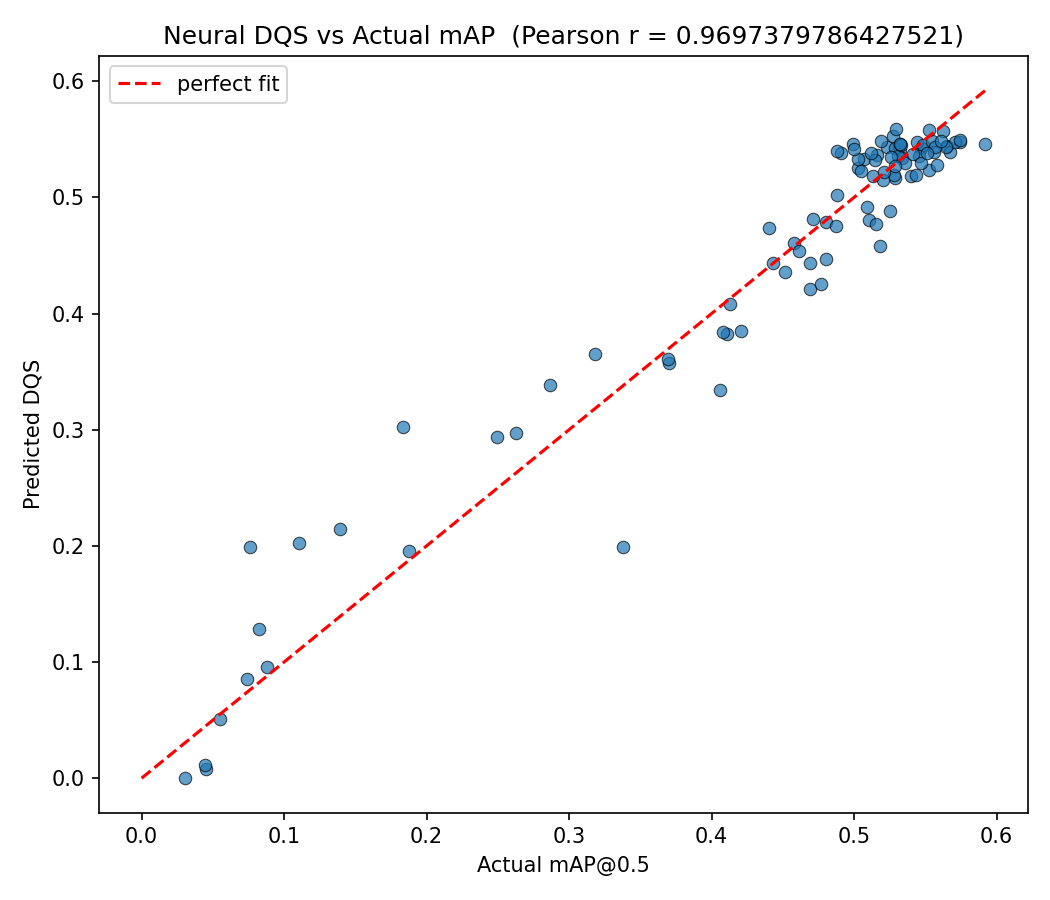
\includegraphics[width=0.7\textwidth]{figures/dqs_scatter.png}
\caption{Neural DQS predicted mAP vs.\ actual mAP@0.5 across 96 controlled
degradation variants of COCO128. Pearson $r=0.929$. The red dashed line
indicates perfect prediction.}
\label{fig:scatter}
\end{figure}

\begin{table}[h]
\centering
\caption{Neural DQS fit statistics ($n=96$).}
\begin{tabular}{@{}lc@{}}
\toprule
Metric & Value \\
\midrule
Train Pearson $r$ & 0.970 \\
\textbf{CV Pearson $r$ ($k=5$)} & \textbf{0.929} \\
CV $R^2$ & 0.854 \\
CV MSE & 0.0033 \\
\bottomrule
\end{tabular}
\end{table}

Table~\ref{tab:feature-corr} reports the Pearson correlation between each of
the six individual features and mAP@0.5.

\begin{table}[h]
\centering
\caption{Per-feature Pearson correlation with mAP@0.5 ($n=96$).}
\label{tab:feature-corr}
\begin{tabular}{@{}lc@{}}
\toprule
Feature & $r$ \\
\midrule
CD --- CLIP Diversity & $+0.892$ \\
IQ --- Image Quality  & $+0.661$ \\
LD --- Lighting Diversity & $+0.264$ \\
CB --- Class Balance  & $-0.140$ \\
PD --- Pose Diversity & $-0.067$ \\
AQ --- Annotation Quality & $-0.042$ \\
\bottomrule
\end{tabular}
\end{table}

These results indicate that Neural DQS is a strong predictor of mAP (CV
$r=0.929$, $p<0.001$), with CLIP Diversity as the single most important
feature.

\subsection{Ablation Study --- DQS Feature Ablation}
\label{sec:dqs-ablation}

Table~\ref{tab:ablation} reports a leave-one-feature-out ablation on the
96-variant benchmark (CV Pearson $r$, $k=5$).

\begin{table}[h]
\centering
\caption{Leave-one-out feature ablation (CV Pearson $r$, $k=5$).}
\label{tab:ablation}
\begin{tabular}{@{}lcc@{}}
\toprule
Configuration & CV $r$ & $\Delta r$ \\
\midrule
\textbf{Full model (6 features)} & \textbf{0.929} & --- \\
w/o CD (CLIP Diversity) & 0.679 & $-0.250$ \\
w/o LD (Lighting Diversity) & 0.923 & $-0.006$ \\
w/o PD (Pose Diversity) & 0.925 & $-0.004$ \\
w/o IQ (Image Quality) & 0.925 & $-0.004$ \\
w/o AQ (Annotation Quality) & 0.928 & $-0.001$ \\
w/o CB (Class Balance) & 0.938 & $+0.009$ \\
\bottomrule
\end{tabular}
\end{table}

Removing CD drops CV $r$ by $0.250$ --- from $0.929$ to $0.679$ ---
confirming that CLIP-space semantic diversity is the single most critical
predictor. All other features contribute modestly; CB slightly \emph{hurts}
the model, since COCO128 is nearly perfectly class-balanced and provides
little variance for this feature to exploit.

We note that Section~\ref{sec:main-table} separately reports an end-to-end
\emph{system}-level comparison (Manual / YOLO-only / ADB / ADB+AL) on the
COCO2017 motorcycle subset, and Section~\ref{sec:pipeline-ablation}
complements it with a full component-wise ablation of the ADB
\emph{pipeline} itself (w/o SAM2, w/o CLIP-verify, and both).

\subsection{DQS Feature Importance}

Figure~\ref{fig:shap} shows the mean absolute SHAP value for each feature
across all 96 variants.

\begin{figure}[h]
\centering
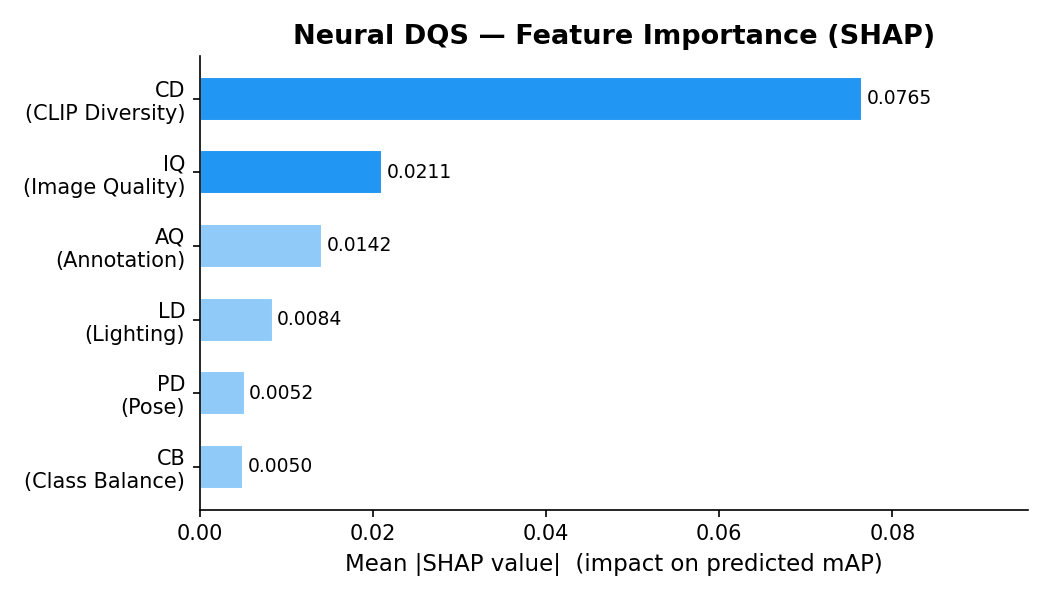
\includegraphics[width=0.7\textwidth]{figures/dqs_shap.png}
\caption{SHAP feature importance (mean $|\phi|$) for Neural DQS across 96
COCO128 degradation variants.}
\label{fig:shap}
\end{figure}

\begin{table}[h]
\centering
\caption{SHAP mean $|\phi|$ (impact on predicted mAP).}
\begin{tabular}{@{}lc@{}}
\toprule
Feature & Mean $|\phi|$ \\
\midrule
CD --- CLIP Diversity & \textbf{0.0765} \\
IQ --- Image Quality  & 0.0211 \\
AQ --- Annotation Quality & 0.0142 \\
LD --- Lighting Diversity & 0.0084 \\
PD --- Pose Diversity & 0.0052 \\
CB --- Class Balance & 0.0050 \\
\bottomrule
\end{tabular}
\end{table}

SHAP confirms the ablation finding: CD dominates, with an importance
3.6$\times$ larger than the second-ranked feature (IQ). Notably, AQ ranks
third in SHAP importance despite its near-zero Pearson correlation
($r=-0.042$), suggesting that annotation completeness captures a non-linear
quality signal --- penalizing missing annotations sharply once completeness
falls below some operating regime, rather than varying smoothly with mAP.

\section{Conclusion}
\label{sec:conclusion}

\subsection{Summary}

We presented ADB, an automated, end-to-end framework for constructing
YOLO-compatible object detection datasets from unlabeled images. Our three
main contributions are: (1) a three-stage annotation pipeline (YOLOv11
$\to$ SAM2 $\to$ zero-shot semantic verification) that requires no manual
annotation; (2) Neural DQS, a learned dataset quality score that predicts
post-training mAP from six interpretable features with cross-validated
Pearson $r=0.929$; and (3) an active learning loop that uses the same
pipeline to automatically re-annotate the most uncertain pool images. On a
597-image COCO2017 motorcycle subset, ADB's fully automated annotations reach
94.2\% of the Manual-annotation mAP@0.5 with zero labeling effort, and a
single active-learning iteration closes this gap entirely.

\subsection{Limitations}
\label{sec:limitations}

\begin{itemize}
\item \textbf{Class vocabulary bound by Stage 1.} The three-stage pipeline's
  proposal stage uses a COCO-pretrained YOLOv11 detector. While Stage 2
  (SAM2) is class-agnostic and Stage 3 (CLIP / Vision-LLM verification) is
  zero-shot with respect to class names, Stage 1 can currently only propose
  candidate boxes for object classes within COCO's 80-category vocabulary.
  Motorcycle was selected as a representative single class from this
  vocabulary for controlled experimentation, not as a hard-coded
  restriction --- but classes outside COCO's vocabulary cannot currently be
  annotated by ADB.
\item \textbf{Single-class proof of concept.} Our end-to-end system
  evaluation (Section~\ref{sec:adb-eval}) is conducted on a single-class
  (motorcycle) detection task. Multi-class and instance-segmentation settings
  may exhibit different trade-offs between SAM2 refinement and CLIP-verify
  rejection rates.
\item \textbf{Single training distribution for Neural DQS.} Neural DQS is
  trained exclusively on controlled degradations of COCO128. As a first
  cross-domain check, we apply the trained model (no retraining) to the 7
  single-class motorcycle dataset variants from
  Section~\ref{sec:pipeline-ablation} and correlate the predicted score
  against each variant's actual mean mAP@0.5 (3 seeds, 50 epochs). The
  cross-domain Pearson correlation is $r=0.617$ ($n=7$), versus $r=0.929$
  in-domain (Table~\ref{tab:dqs-correlation}). The model thus retains a
  moderate-to-strong positive correlation out-of-domain but with
  substantially reduced strength, indicating that its learned feature
  weights --- tuned for COCO128's 80-class, multi-object degradation
  patterns --- only partially transfer to a single-class, sparsely-populated
  dataset. Generalization to other domains (e.g., medical or aerial imagery)
  with substantially different image resolutions remains unevaluated.
\item \textbf{LLM verification not evaluated end-to-end.} The Vision-LLM
  verification backend (Qwen-VL-Chat / LLaVA) is implemented but, due to the
  CPU-only experimental setup, all reported ADB results use the CLIP
  zero-shot backend as a substitute for this stage.
\end{itemize}

\subsection{Future Work}
\label{sec:future}

\begin{enumerate}
\item \textbf{Open-vocabulary proposal generation.} Replacing the Stage-1
  YOLOv11 detector with an open-vocabulary detector such as Grounding
  DINO~\citep{liu2023grounding} or YOLO-World~\citep{cheng2024yoloworld}
  would remove the COCO-80 class restriction discussed in
  Section~\ref{sec:limitations}, allowing ADB to annotate arbitrary classes
  specified purely via natural language --- directly realizing the original
  ``natural language $\to$ dataset'' goal of the system.
\item \textbf{Multi-class and instance segmentation.} Extending the
  end-to-end evaluation of Section~\ref{sec:adb-eval} to multi-class
  detection and instance segmentation tasks.
\item \textbf{A DQS meta-dataset.} Constructing a larger, cross-domain
  training set for Neural DQS spanning multiple base datasets and domains, to
  evaluate and improve its generalization beyond COCO128. The cross-domain
  drop from $r=0.929$ to $r=0.617$ observed in
  Section~\ref{sec:limitations} suggests that including non-COCO,
  single-class data during training could meaningfully narrow this gap.
\item \textbf{Lightweight local Vision-LLM verification.} Evaluating the
  Vision-LLM verification backend end-to-end with a locally-served,
  lightweight model, and comparing its rejection behavior to the CLIP
  zero-shot backend used in this paper.
\item \textbf{Integration with existing annotation platforms.} Exporting ADB
  datasets directly into platforms such as Roboflow or Label Studio for
  human review of low-confidence annotations.
\end{enumerate}

\bibliographystyle{plainnat}
\bibliography{references}

\end{document}
